40. Сумма внешних углов любого многоугольника равна $360^\circ,$ а сумма его внутренних углов равна $(n-2)\cdot180^\circ,$ где $n$ это количество вершин. Значит, $(n-2)\cdot180^\circ=3\cdot360^\circ,\ n=8.$\newpage

\noindent41. \begin{figure}[ht!]
\center{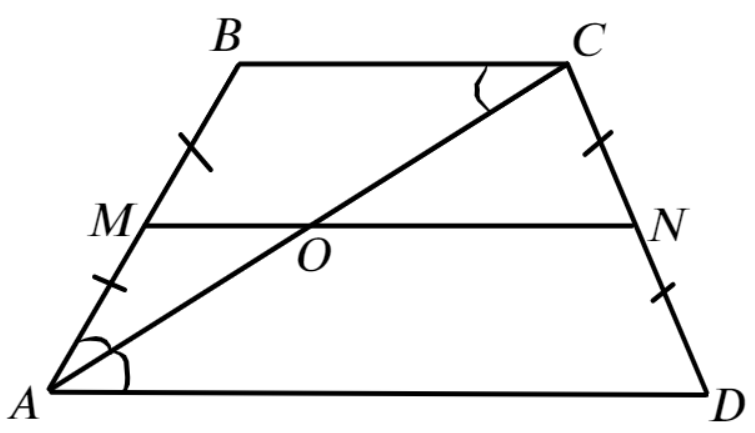
\includegraphics[scale=0.35]{g9-41.png}}
\end{figure}\\
Углы $BAC$ и $CAD$ равны так как $AC$ --- биссектриса, а углы $CAD$ и $BCA$ равны как накрест лежащие, значит $\angle BAC=\angle BCA$ и треугольник $ABC$ равнобедренный, $AB=BC.$ Прямая $MN$ параллельна основаниям трапеции и проходит через середины сторон $AB$ и $CD,$ значит отрезки $MO$ и $ON$ являются средними линиями треугольников $ABC$ и $ACD$ соответственно. Тогда $BC=2MO=2\cdot7,5=15$см и $AB=BC=CD=15$см (так как трапеция равнобедренная), а $AD=2AN=2\cdot12,5=25$см.\\
